\section{dirtree 结构图}
\subsection{dirtree 代码}
\index{宏包!dirtree}
\index{命令!\verb$\dirtree$}
使用 dirtree 宏包。如下图所示

\dirtree{%
.1 /.
.2 bin.
.2 home.
.3 jeancome.
.4 texmf.
.5 tex.
.6 latex.
.7 dirtree.
.3 jeancomeson.
.3 jeancomedaughter.
.2 usr.
.3 bin.
.3 games.
.4 fortunes.
.3 include.
.3 local.
.4 bin.
.4 share.
.5 texmf.
.6 fonts.
.6 metapost.
.6 tex.
.3 share.
}
对应代码如下:
\begin{lstlisting}
\dirtree{%
.1 /.
.2 bin.
.2 home.
.3 jeancome.
.4 texmf.
.5 tex.
.6 latex.
.7 dirtree.
.3 jeancomeson.
.3 jeancomedaughter.
.2 usr.
.3 bin.
.3 games.
.4 fortunes.
.3 include.
.3 local.
.4 bin.
.4 share.
.5 texmf.
.6 fonts.
.6 metapost.
.6 tex.
.3 share.
}
\end{lstlisting}




\subsection{dirtree 参数设计}
\begin{description}
  \item[DTstyle] 结点文字的属性
  \item[DTcomment] 右侧注释的内容
  \item[DTstylecomment] 右侧注释文字的属性
  \item[DTsetlength] 如下图所示
\begin{figure}[H]
  \centering
  % Requires \usepackage{graphicx}
  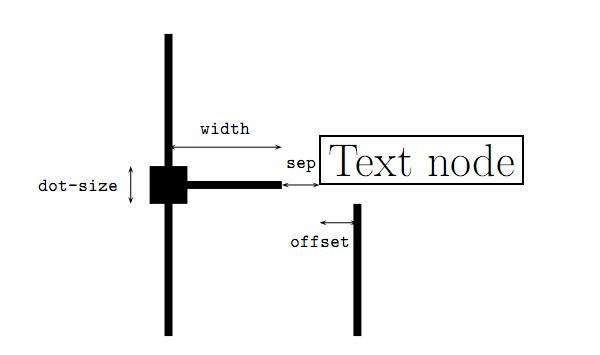
\includegraphics[width=10cm]{dirtree_length}\\
  \caption{dirtree 长度设置}\label{dirtree_length}
\end{figure}

\begin{cmd}[label= 长度设置命令]
    \DTsetlength{offset}{width}{sep}{rule-width}{dot-size}
默认值如下:
• offset=0.2em
• width=1em
• sep=0.2em
• rule-width=0.4pt
• dot-size=1.6pt
\end{cmd}
  \item[DTbaselineskip] 基线设置

\begin{cmd}[label= 基线设置命令]
\setlength{\DTbaselineskip}{20pt}
\DTsetlength{1em}{3em}{0.1em}{1pt}{4pt}
\end{cmd}
\end{description}

\renewcommand*\DTstylecomment{\rmfamily\color{green}\textsc}
\renewcommand*\DTstyle{\ttfamily\textcolor{red}}
\dirtree{%
.1 /.
.2 bin.
.2 home.
.3 jeancome.
.4 texmf.
.5 tex.
.3 jeancomeson\DTcomment{Guillaume}.
.3 jeancomedaughter\DTcomment{Mathilde}.
.2 usr.
.3 bin.
}


\lstset{language=[LaTeX]TeX}
\begin{lstlisting}
\dirtree{%
.1 /.
.2 bin.
.2 home.
.3 jeancome.
.4 texmf.
.5 tex.
.3 jeancomeson\DTcomment{Guillaume}.
.3 jeancomedaughter\DTcomment{Mathilde}.
.2 usr.
.3 bin.
}
\end{lstlisting}


\dirtree{%
.1 /.
.2 bin\ldots{}\begin{minipage}[t]{5cm}
This directory hold sexecutable files (binary
files or link on binary files){.}
\end{minipage}.
.2 home\ldots{}\begin{minipage}[t]{5cm}
jeancome\\
guillaume\\
mathilde\\
\end{minipage}.
.4 texmf.
}

\begin{lstlisting}

\dirtree{%
.1 /.
.2 bin\ldots{}\begin{minipage}[t]{5cm}
This directory hold sexecutable files (binary
files or link on binary files){.}
\end{minipage}.
.2 home\ldots{}\begin{minipage}[t]{5cm}
jeancome\\
guillaume\\
mathilde\\
\end{minipage}.
.4 texmf.
}
\end{lstlisting}
